\documentclass[12pt]{article}
\usepackage[T1]{fontenc}
%\usepackage[latin9]{inputenc}
\usepackage[utf8]{inputenc}
\usepackage[english]{babel}
\usepackage{amsmath}
%\usepackage{halloweenmath}
\usepackage{amsfonts}
\usepackage{amssymb}
%\usepackage{setspace}
\usepackage{rotating}
\usepackage{graphics}
\usepackage{eurosym}
\usepackage[round]{natbib}
%\usepackage{graphicx}
%\usepackage{float} 				%allows you to float images
\usepackage{latexsym}
%\usepackage{bbding}
%\usepackage {moresize}
\usepackage{listings}
\usepackage{bbding}
\usepackage{blindtext}
\usepackage{hhline}
\usepackage{tikz}
\usetikzlibrary{trees}
%\usetikzlibrary{shapes,backgrounds}
%\usepackage{pgfplots}
%\usetikzlibrary{arrows}
\usepackage{enumitem}
%\doublespacing
%\usepackage{geometry}
\usepackage{amsthm}
\usepackage{color}
%\usepackage{array,multirow}
\usepackage{subcaption}
%\usepackage{pst-plot}
%	\psset{xunit=15mm}
%\geometry{verbose,tmargin=1in,bmargin=1in,lmargin=.5in,rmargin=.5in}
\setlength{\parskip}{\bigskipamount}
\setlength{\parindent}{0pt}
\usepackage{multicol}


\newenvironment{problem}[3][Problem]{\begin{trivlist}
\item[\hskip \labelsep {\bfseries #1}\hskip \labelsep {\bfseries #2.}]}{\end{trivlist}}

\newcommand{\barr}{\bar{r}}
\newcommand{\ddx}{\frac{d}{dx}}
\newcommand{\infsum}{\sum_{n=1}^{\infty }}

\title{Problem Set 12 \thanks{Problems:17.4.1, 17.22, 17.23, 18.7, 18.8, 18.5, 18.22}}
\author{Ian McGroarty \\
	Course Number: 555.444 \\
}
\date{November 19, 2019}

\begin{document}

\maketitle
%%%%%%%%%%%%%%%%%%%%%%%%%%%%%%%%%%%%%%%%%%%%%%%%%%%%%%%%
%%%%%%%%%%%%%%%%%%%%%%%%%%%%%%%%%%%%%%%%%%%%%%%%%%%%%%%%
%%%%%%%%%%%%%%%%%%%%%%%%%%%%%%%%%%%%%%%%%%%%%%%%%%%%%%%%

\newpage
\begin{problem}{15.4}. $S_0 = 0.80, k= 0.79, \sigma = 0.12, r= 0.06, r_f = 0.08, T=4 \ mon$ With these parameters we can find, $\delta t = 2$, $u=e^{\sigma \cdot \sqrt{\delta t}} = e^{0.12 \cdot \sqrt{2/12}} = 1.05$ and thus $d = 1/u = 1/(1.05) = 0.952$ and $a=e^{(r-r_f) \delta t} = e^{(0.06-0.08)*2}=0.961.$ We can now find $p=\frac{a-d}{u-d} = \frac{0.961 - 0.952}{1.05-0.952} = 0.454$ The binomial tree show below shows the value of the European call and American Call options. 	

\begin{figure}[h!]
\centering
\begin{subfigure}{0.4\textwidth}
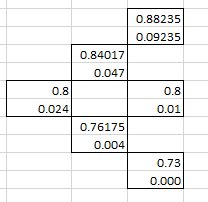
\includegraphics[width=\linewidth]{mod12_p174a.png}
\caption{European Call}
\end{subfigure}
\begin{subfigure}{0.4\textwidth}
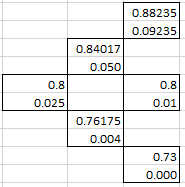
\includegraphics[width=\linewidth]{mod12_p174b.png}
\caption{American Put}
\end{subfigure}
\end{figure}
\end{problem}

\begin{problem}{17.22}. Can an option on the yen-euro exchange rate be created from two options, one on the dollareuro exchange rate, and the other on the dollar-yen exchange rate? Explain your answer.

Okay so the obvious answer here is yes and the way to do it would be to, first buy a call sell a put on dollar-yen rates then do the same for euro-yen rates. But I want to talk about this a different way that I makes more sense to me. It must be the case that the following holds: $$\frac{Yen}{Dollar}\cdot {Dollar}{Euro}= \frac{Yen}{Euro}$$
The arbitrage opportunities available if this equality were not true are fairly obvious. So the must exist a series of options fixing the exchange rates against the dollar that allow you to fix the exchange rate to the Yen/Euro. 

\end{problem}
\begin{problem}{17.23}. DerivaGem
\end{problem}


\begin{problem}{18.7}. adfgasdf
\end{problem}

\begin{problem}{18.8}. Suppose you buy a put option contract on October gold futures with a strike price of \$1400 per ounce. What happens when you exercise for \$1380. 

You\rq{}ll get a futures contract + $(1400-1380)*100 = \$2,000$ cash money. 
\end{problem}

\begin{problem}{18.15}. $F_0= 70, \sigma = 20\% , r= 0.06, K=65$. 
\begin{align*}
d_1 &= \frac{ln(F_0/K) + (\sigma^2/2)(T)}{\sigma \sqrt{T}}  && \text{(pg 388)} \\
&= \frac{ln(70/65) + (0.2^2/2)((5/12))}{0.2 \sqrt{(5/12)}} = 0.6386 \\
d2 &= d_1 - \sigma \sqrt{T}  \\
&= 0.6386 - 0.6\sqrt{5/12} = 0.5905 \\
p &= e^{-rT}[KN(-d_2) - F_0N(-d_1) && \text{Eqn. 18.8 (pg. 388)} \\
p &= e^{-0.06*(5/12)}[65\cdot N(-0.5905) -  70 \cdot N(-0.6386)] \\
p &= 1.498 
\end{align*}
\end{problem}

\begin{problem}{18.22}. $F_0 = 40$ If is known that at the end of three months the price will be either 35 or 45. What is the value of a three month European call option an the futures with a strike price of 42 if the risk free interest rate is 7\%?

$F_u \cdot u = 40 \cdot u = 45 \rightarrow u = 1.125 \rightarrow d= 0.875$ So, $p = \frac{1-d}{u-d} = 0.5$ So,
\begin{align*}
f&=e^{-rT}[p\cdot f_u + (1-p)\cdot f_d] && \text{Eqn. 18.9 (pg 391)} \\
f&=e^{-0.06 (3/12)}[0.5\cdot 45 + 0.5\cdot 35] = 1.474 
\end{align*}
\end{problem}

\end{document}
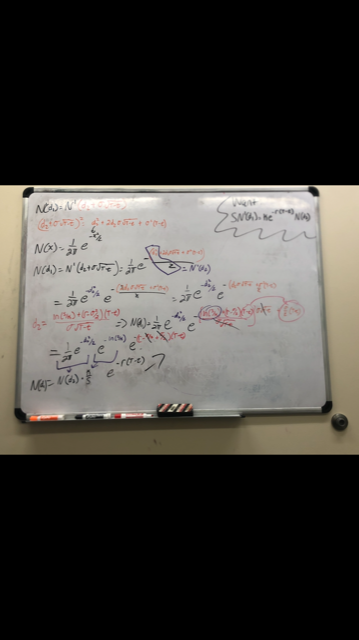
\includegraphics[width=\linewidth]{mod11_p1517b.png}

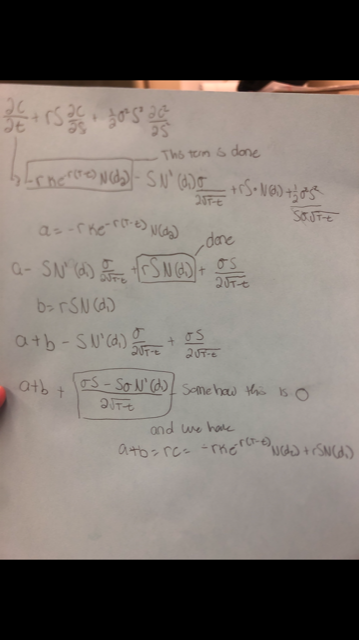
\includegraphics[width=\linewidth]{mod11_p1517f.png}
